\documentclass{standalone}
\usepackage{tikz}
\usetikzlibrary{calc} % 坐标计算库
\usetikzlibrary{patterns} % 阴影填充库
\usepackage{pgfplots} % 绘图库
\usepgfplotslibrary{fillbetween} % 区域阴影
\pgfplotsset{compat=1.18} % 设置 pgfplots 版本
\usetikzlibrary{patterns.meta} % 图案库

% 常量声明
\newcommand{\xmin}{0}
\newcommand{\xmax}{7}
\newcommand{\ymin}{-15}
\newcommand{\ymax}{4}
\newcommand{\domainstart}{0}
\newcommand{\domainend}{6}

\begin{document}

\begin{tikzpicture}
    % Shear Diagram
    \begin{axis}[
            axis lines=middle, % 学校式坐标轴
            axis line style={thick},
            xlabel={$x(m)$},
            xlabel style={right},
            ylabel={$V(kN)$},
            ylabel style={above},
            xtick={\domainend},
            xticklabel style={anchor=south, yshift=4pt},
            ytick={-2},
            xmin=\xmin, xmax=\xmax,
            ymin=\ymin, ymax=\ymax,
            domain=0:\domainend,
        ]
        % 定义函数和x轴
        \addplot[name path=A, thick] {-2};
        \addplot[name path=B] {0};
        % 填充两者之间的区域
        \addplot[
            pattern={Lines[angle=45, distance=6pt]},
        ] fill between [of=A and B];
        % 添加标识线或点
        \draw[thick] (axis cs:6,0) -- (axis cs:6,-2);
    \end{axis}

\end{tikzpicture}

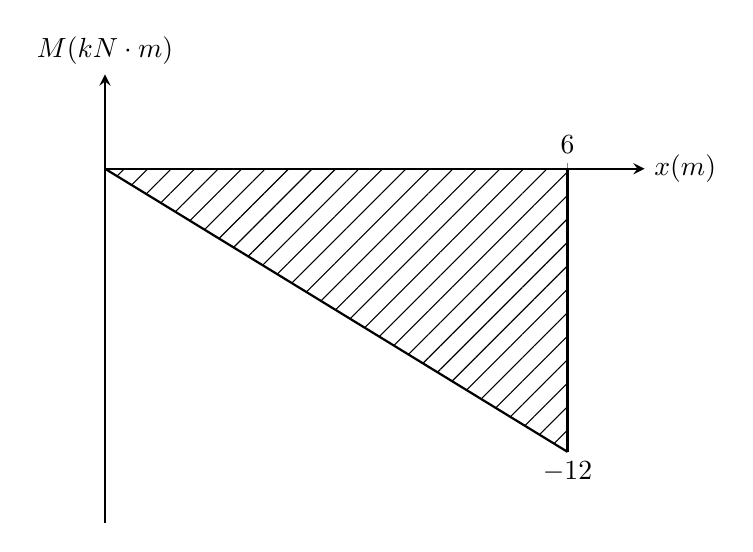
\begin{tikzpicture}
    % Moment Diagram
    \begin{axis}[
            axis lines=middle, % 学校式坐标轴
            axis line style={thick},
            xlabel={$x(m)$},
            xlabel style={right},
            ylabel={$M(kN \cdot m)$},
            ylabel style={above},
            xtick={\domainend},xticklabel style={anchor=south, yshift=4pt},
            ytick=\empty,
            xmin=\xmin, xmax=\xmax,
            ymin=\ymin, ymax=\ymax,
            domain=0:6,
        ]
        % 定义函数和x轴
        \addplot[name path=A, domain=0:\domainend, thick] {-2*x};
        \addplot[name path=B, domain=0:\domainend] {0};
        % 填充两者之间的区域
        \addplot[
            pattern={Lines[angle=45, distance=6pt]},
        ] fill between [of=A and B];
        % 添加标识线或点
        \draw[thick] (axis cs:\domainend,0) -- (axis cs:\domainend,-12);
        \node at (axis cs:\domainend,-12) [below] {$-12$};
    \end{axis}

\end{tikzpicture}

\end{document}